%!TEX root=../draft.tex
%\vspace{-6pt}
\section{Compiling to the Overlay}
\label{ch4_tool}
There are two separate design processes for mapping an application to an overlay. The first is the overlay implementation which is carried out offline using the conventional FPGA design flow. 
At power-on, the bitstream (consisting of the overlay, memory and communication interfaces, and any other components) is used to configure the FPGA.
The second involves mapping the application kernel to the overlay.
To allow for fast vendor independent mapping to the overlay we developed our own mapping tool flow.
This involves, DFG extraction from high-level compute kernels, scheduling the DFG nodes onto the overlay, and finally, instruction generation for each FU. This is typically done offline, however it could also be performed as part of a just-in-time mapping strategy.
On Zynq, the ARM processor loads the kernel configuration into the overlay pipeline and initiates kernel execution.
Our mapping flow is described below using the previous example.

\textbf{\textit{Kernel Mapping:}} The open source HercuLeS HLS tool~\cite{kavvadias2013hardware} is used to transform a `C' description of the compute kernel to a DFG description, where nodes represent operations and edges represent data flow between operations, as shown in Fig.~\ref{dfg}.
For the V1 and V2 based overlays, ASAP scheduling is used which results in no data dependencies between operations at the same scheduling stage, as in~\cite{li2016area}, with nodes in each scheduling stage then being allocated to a single V1 or V2 FU for execution. 
The set of instructions from the sequenced DFG is identified, then the cycle-by-cycle execution pattern is formed which interleaves load/store and arithmetic/ALU operations, as shown in Table~\ref{schedule}. 
For the `gradient' benchmark, the II is reduced from 11 (in~\cite{li2016area}) to 6 (V1) or 3 (V2) with the same ASAP scheduling.
This translates to a throughput of 0.59 Giga-operations/s (GOPS) for the V1 based overlay with a latency of 86.8 ns (1.11 GOPS and 92.4 ns for V2). 
Lastly the 32-bit FU instructions are generated.

\begin{comment}
An overlay has two separate design processes: Overlay implementation on the FPGA and application mapping to the overlay.
While the design and implementation of the overlay relies on the conventional hardware design flow using vendor tools, this process is done offline, once only, and so does not impact the compute kernel implementation of an application. 
We then use an in-house automated compilation flow to provide a rapid, vendor independent, mapping to the overlay.
The mapping process comprises DFG extraction from high-level compute kernels, scheduling of the DFG nodes onto the overlay, and finally, the instruction generation for each FU. This is also done offline.
Then at power-on the bitstream for the overlay, and any other unrelated hardware components, is used to configure the FPGA. Subsequent to this, the ARM processor loads the kernel configuration into the overlay pipeline and initiates kernel execution.
Our mapping flow is described below using the previous example.


\textbf{\textit{HLL to DFG Conversion:}} The tool transforms a `C' description of the compute kernel to a DFG text description, where nodes represent operations and edges represent data flow between operations, as shown in Fig. 1(b).


\textbf{\textit{Operation Scheduling:}} Scheduling is used to generate a sequenced DFG, with nodes in each scheduling stage being allocated to a single FU for execution. 
Here, the set of instructions from the sequenced DFG is identified, then the cycle-by-cycle execution pattern is formed as shown in Table~\ref{schedule}, and lastly the 32-bit FU instructions are generated.
\end{comment}


\begin{table}[b]
	\renewcommand{\arraystretch}{1}
	\caption{First 32 cycles of the `gradient' schedule (II=6).}
	\label{schedule}
	\centering
	\scriptsize
	\resizebox{\columnwidth}{!}{
		\begin{tabular}{lllllllll}
			\toprule
			cycle & \multicolumn{2}{c}{FU0} & \multicolumn{2}{c}{FU1} & \multicolumn{2}{c}{FU2} & \multicolumn{2}{c}{FU4} \\ \midrule
			1     & Load R0 &               &         &               &         &               &         &  \\
			2     & Load R1 &               &         &               &         &               &         &  \\
			3     & Load R2 &               &         &               &         &               &         &  \\
			4     & Load R3 &               &         &               &         &               &         &  \\
			5     & Load R4 &               &         &               &         &               &         &  \\
			6     &         & SUB (R0 R2)   &         &               &         &               &         &  \\
			7     & Load R0 & SUB (R1 R2)   &         &               &         &               &         &  \\
			8     & Load R1 & SUB (R2 R3)   &         &               &         &               &         &  \\
			9     & Load R2 & SUB (R2 R4)   & Load R0 &               &         &               &         &  \\
			10    & Load R3 &               & Load R1 &               &         &               &         &  \\
			11    & Load R4 &               & Load R2 &               &         &               &         &  \\
			12    &         & SUB (R0 R2)   & Load R3 &               &         &               &         &  \\
			13    & Load R0 & SUB (R1 R2)   &         & SQR (R0 R0)   &         &               &         &  \\
			14    & Load R1 & SUB (R2 R3)   &         & SQR (R1 R1)   &         &               &         &  \\
			15    & Load R2 & SUB (R2 R4)   & Load R0 & SQR (R2 R2)   &         &               &         &  \\
			16    & Load R3 &               & Load R1 & SQR (R3 R3)   & Load R0 &               &         &  \\
			17    & Load R4 &               & Load R2 &               & Load R1 &               &         &  \\
			18    &         & SUB (R0 R2)   & Load R3 &               & Load R2 &               &         &  \\
			19    & Load R0 & SUB (R1 R2)   &         & SQR (R0 R0)   & Load R3 &               &         &  \\
			20    & Load R1 & SUB (R2 R3)   &         & SQR (R1 R1)   &         & ADD (R0 R1)   &         &  \\
			21    & Load R2 & SUB (R2 R4)   & Load R0 & SQR (R2 R2)   &         & ADD (R2 R3)   &         &  \\
			22    & Load R3 &               & Load R1 & SQR (R3 R3)   & Load R0 &               &         &  \\
			23    & Load R4 &               & Load R2 &               & Load R1 &               & Load R0 &  \\
			24    &         & SUB (R0 R2)   & Load R3 &               & Load R2 &               & Load R1 &  \\
			25    & Load R0 & SUB (R1 R2)   &         & SQR (R0 R0)   & Load R3 &               &         & ADD (R0 R1)   \\
			26    & Load R1 & SUB (R2 R3)   &         & SQR (R1 R1)   &         & ADD (R0 R1)   &         &  \\
			27    & Load R2 & SUB (R2 R4)   & Load R0 & SQR (R2 R2)   &         & ADD (R2 R3)   &         &  \\
			28    & Load R3 &               & Load R1 & SQR (R3 R3)   & Load R0 &               &         &  \\
			29    & Load R4 &               & Load R2 &               & Load R1 &               & Load R0 &  \\
			30    &         & SUB (R0 R2)   & Load R3 &               & Load R2 &               & Load R1 &  \\
			31    & Load R0 & SUB (R1 R2)   &         & SQR (R0 R0)   & Load R3 &               &         & ADD (R0 R1)   \\
			32    & Load R1 & SUB (R2 R3)   &         & SQR (R1 R1)   &         & ADD (R0 R1)   &         &  \\ \bottomrule
		\end{tabular}
	}
\end{table}

Typically, most of the existing CGRA architectures adopt Modulo scheduling~\cite{rau1994iterative}, or a derivative algorithm, to achieve a minimum II. 
However, Modulo scheduling is based on the assumption that each operation node is executed in 1 cycle and the transfer of data between two arbitrary FUs completes in 1 cycle, which is not realistic for highly pipelined architectures. 
Instead, for a fixed depth overlay we use an iterative greedy scheduling strategy which groups DFG nodes at each scheduling step into clusters and then adds DFG nodes along the critical path from subsequent clusters, while balancing the II across all clusters.
The number of scheduling clusters is equal to the overlay depth.
Due to space constraints, the scheduling algorithm will not be discussed further.
%, which in this case is 8.

As an example of fixed depth overlay scheduling, consider the `qspline' benchmark, of Fig.~\ref{qspline}. Here, the critical path is 8 and we map to a depth 4 overlay (4 FUs). Scheduling produces the 4 instruction clusters shown in Fig.~\ref{qspline} (using red dashes). NOPs (equal to IWP-1) must be added between dependant instructions (DFG nodes) unless other non-dependant instructions can be scheduled in between. For example, in the first (top) cluster, Node 17 is scheduled, followed by 13, 25, 9, 20, and 12, before 15 is scheduled. Hence, the dependency between 17 and 15 is resolved and no NOPs are inserted. 
Similarly for the 2nd cluster, scheduling as: 14, 26, 21, 10, 16, 11, 27, 22, resolves dependencies 14-11, 26-27, and 21-22, for all overlay versions. In cluster three, scheduling as: 18, 24, 28, 23, 19, 30, 8, resolves all dependencies for the V4 and V5 overlays, but not for the V3 overlay, which with an IWP of 5 requires 4 operations between dependant nodes. Hence, a single NOP must be added between 23 and 19 which then resolves all 4 sets of dependant instructions.
For the 4th cluster, graph balancing is performed, and the two additions scheduled, followed by IWP-1 NOPs before the final addition.
%(equal to IWP-1) must be added between 31 and 32, and 32 and 29. 

%Here the V3 overlay has an II of 17, with a throughput of 0.45 Giga-operations/s (GOPS) and the latency of 135ns, while the V4 overlay has 14, 0.43 GOPS and 151ns, respectively (compared to the depth 8 V1 overlay with 11, 0.69 GOPS and 234ns, respectively). 

The consequences of a fixed depth overlay are an increase in the II with a corresponding reduction in the throughput, but with a significant reduction in the latency. For the `qspline' benchmark, the V3 overlay has an II of 15, with a throughput of 0.51 GOPS and a latency of 125 ns, while the V4 overlay has an II of 14, a throughput of 0.43 GOPS and a latency of 148 ns. This compares to the depth 8 V1 overlay with an II of 11, a throughput of 0.69 GOPS and a latency of 234ns. 
%It should be noted, that in some cases, limiting the depth of the overlay and properly balancing the schedule between stages actually results in a reduction in the II, compared to the simple ASAP schedule used in the V1 overlay, as can be seen in Table~\ref{benchmarks}. 



\begin{comment}
Therefore, this paper is focusing on architectural exploration, and an ASAP scheduling is generated for the `gradient' benchmark shown as indicated in Table~\ref{schedule}, which takes advantage of the rotating register file. 
It is applicable to the design of V1 and V2 as there is no data dependency between operations at the same stage.
Similar to the operation scheduling for~\cite{li2016area}, input data coming from the FIFO channel are loaded into the RF of FU0 at the initial 5 cycles (from clock cycle 1 to clock cycle 5).
As soon as loading has completed, FU0 is triggered at the 6th clock cycle and starts executing the 4 SUB instructions using the data from the RF, with a cycle-by-cycle fashion. 
FU0 starts sending the resulting data to FU1 on the 9th clock cycle (due to the 3 stage internal pipeline in the DSP block) and then waits for the cycle to repeat. 
The operations of FU1, FU2 and FU3 are similar to that of FU0, and the result of FU3 is sent back to the output FIFO channel on the 28th clock cycle.
The only difference between the scheduling of V1/V2 and~\cite{li2016area} is that, each FU is able to fetch another set of data from the previous stage without waiting for all the operations to be finished. 
Regarding to the load/store and arithmetic/ALU operations belong to each FU respectively, we find that the maximum value generated from Equation~\ref{II_V1} is 6 for this particular benchmark. 
That means, the II is reduced from 11 (\cite{li2016area}) to 6 (V1) with the same ASAP scheduling.
Similarly, the II of V2 can be further reduced to 3. 


Noted that this simple scheduling may cause conflict on V4 when the data from previous stage and the feedback data are writing to the RF at the same time, the computing operations should be triggered as soon as the necessary data are valid in the RF. 
The order of the instructions also needs to tune to make sure that the feedback data are ready before the execution of associated instructions to avoid NOP insertions.
The `qspline' benchmark is indicated as an example to show the scheduling of V4, shown in Fig.~\ref{qspline}. 
The operation nodes marked as N12, N20, N9, N25, N13, N17 and N15 are clustering into the first schedule stage. 
The second stage consists of operation nodes N10, N21, N26, N14, N27, N11 and N16, while N28, N22, N24, N18, N8, N23, N30 and N19 are grouped into the third stage. 
The last three operation nodes N31, N32 and N29 are scheduled in the final stage. 
In this scheduling, we achieve a significant reduction of the No. of FU from 8 to 4 compared to V1, with a modest penalty of II increase from 11 to 15.
\end{comment}

\begin{figure}[tb]
	\centering
	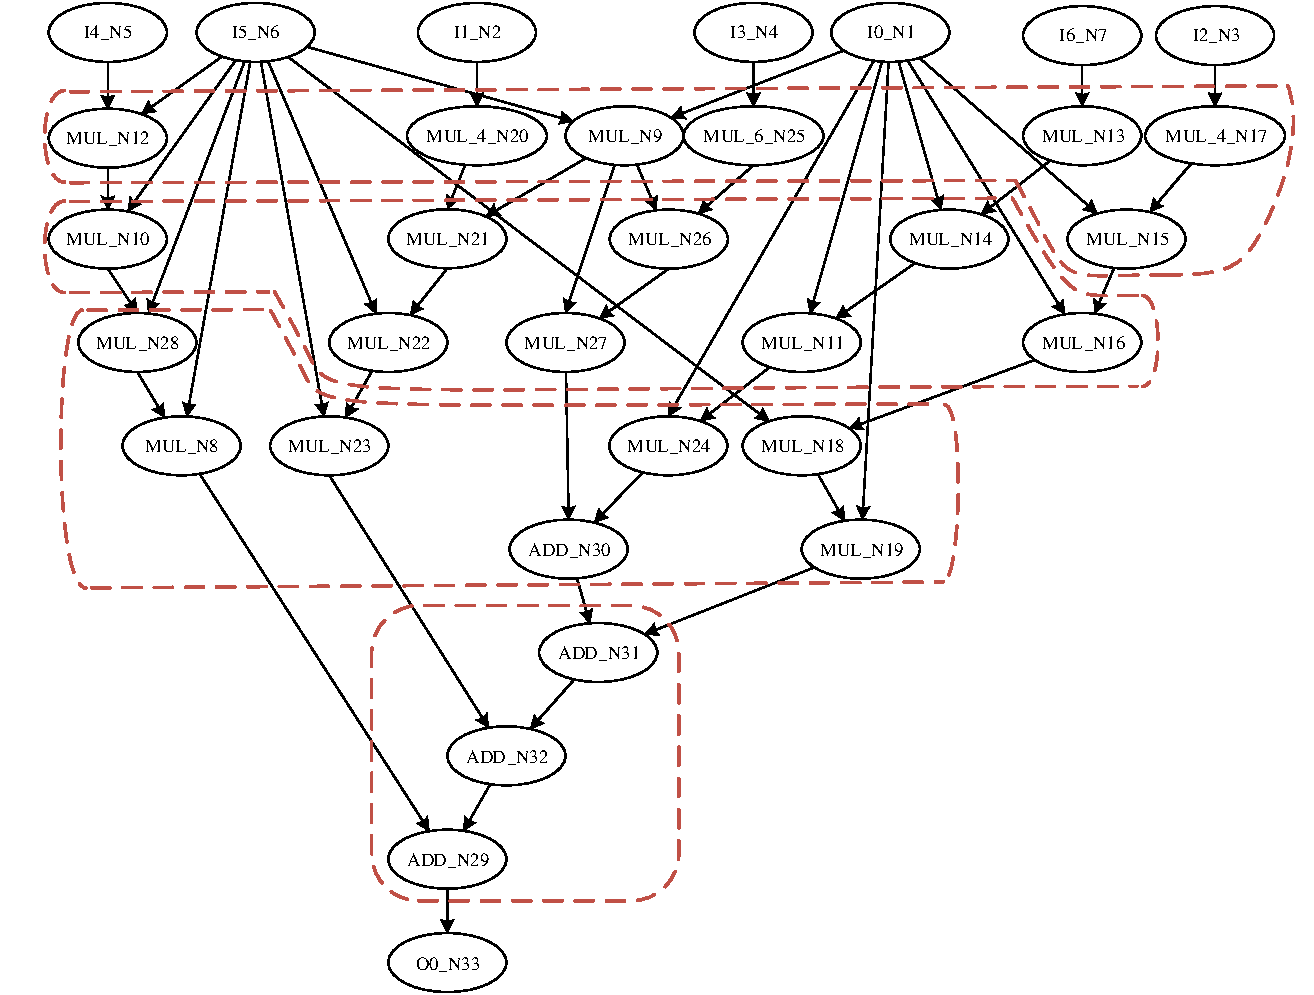
\includegraphics[width=8cm]{figures/Cluster_qspline.pdf}
	\caption{Data flow graph of the `qspline' benchmark.}
	\label{qspline}
\end{figure}



%Section End